\documentclass[a4paper]{article}
\usepackage[english,russian]{babel}
\usepackage[utf8x]{inputenc}
\usepackage[T1]{fontenc}
\usepackage[a4paper,top=2cm,bottom=2cm,left=1cm,right=1cm,marginparwidth=1.75cm]{geometry}
\usepackage{amsmath}
\usepackage{graphicx}

\usepackage[usenames,dvipsnames]{color}

\usepackage{alltt}

\usepackage{listings}
\usepackage{color}

\definecolor{dkgreen}{rgb}{0,0.6,0}
\definecolor{gray}{rgb}{0.5,0.5,0.5}
\definecolor{mauve}{rgb}{0.58,0,0.82}

\lstset{frame=tb,
  language=Octave,
  aboveskip=3mm,
  belowskip=3mm,
  showstringspaces=false,
  columns=flexible,
  basicstyle={\small\ttfamily},
  numbers=none,
  numberstyle=\tiny\color{gray},
  keywordstyle=\color{blue},
  commentstyle=\color{dkgreen},
  stringstyle=\color{mauve},
  breaklines=true,
  breakatwhitespace=true,
  tabsize=3
}

\begin{document}

\begin{center}
    \Large Лабораторная работа по "Уравнениям математической физики" \\
\end{center}

\begin{center}
Выполнил: Пономарев Александр \\
Вариант: 19 \\

\end{center}

\section{Постановка задачи}

\textbf{1. Словесное описание}

Струна конечной длины. Оба конца струны закреплены. Струна подвергается
воздействию распределенной неоднородной силы:

$$
    F(t, x) = ae^{-\frac{(x-x_0)^2}{\gamma^2}}
$$

Параметры:
    плотность струны,
    натяжение струны,
    длина струны,
    амплитуда силы $ a $,
    точка приложения силы $ x_0 $ (внутри струны)
    и характерная ширина её распределения $ \gamma $. \\
\textbf{2. Физический смысл}

Физический смысл задачи описывает колебания струны, которая в начальный момент находилась в покое в положении равновесия и колеблется в результате внешнего воздействия, приложенного к её точке приложения и обеспечивающего перемещение этих концов по заданным законам.

В данной задачи используется волновое уравнение, которое описывает малые поперечные колебания однородной струны, продольные колебания стержня и другие колебательные процессы.

$$u_{tt}-c^2u_{xx}=f(t,x)$$

В случае колебания струны:

$$c^2={T\over \rho_l}, \qquad f(t,x)={F(t,x)\over \rho_l}$$

Где:
\begin{itemize}
    \item $ l $ - длина струны.
    \item $ c $ - фазовая скорость.
    \item $ T $ - сила натяжения струны.
    \item $ \rho_l $ - линейная плотность.
    \item $ h(t,x) $ - плотность распределения внешней силы, дейстующей на струну.
\end{itemize}
\textbf{3. Постановка краевой задачи (Кз)}

Т.к. концы струны закреплены, используем граничные условия первого рода:

$$
    \left\{
        \begin{aligned}
            u(t,0)=0 \\
            u(t,l)=0
        \end{aligned}
    \right.
$$

Введем начальные условия:

$$
    \left\{
        \begin{aligned}
            u(0,x) = \varphi(x) \\
            u_t(0,x) = \psi(x)
        \end{aligned}
    \right.
$$

Где:
\begin{itemize}
    \item $\varphi(x)$ задает начальное положение точек струны.
    \item $\psi(x)$ задает скорость точек струны в начальный момент времени.
\end{itemize}

В итоге получаем краевую задачу:

$$\left\{
    \begin{aligned}
        u_{tt} = c^2u_{xx} + {a \over \rho}e^{-\frac{(x-x_0)^2}{\gamma^2}} \\
        u(t,0) = u(t,l) = 0 \\
        u(0,x) = \varphi(x) \\
        u_t(0,x) = \psi(x)
    \end{aligned}
\right.$$

\newpage

\section{Аналитическое решение задачи}
\textbf{1. Первая вспомогательная задача}

Примем $ f(t,x) = 0 $ и решим следующую краевую задачу:

$$\left\{
    \begin{aligned}
        u_{tt}-c^2u_{xx} = 0 \\
        u(t,0) = u(t,l) = 0  \\
        u(t,0) = \varphi(x)  \\
        u_t(0,x) = \psi(x)
    \end{aligned}
\right.$$

Будем искать решение в виде:

$$
    u(t,x) = T(t)X(x)
$$

Тогда уравнения имеет вид:

$$ X(x)T''(t) - c^2X''(x)T(t) = 0 $$
$$
{X''(x) \over X(x)}={T''(t) \over T(t)}=\lambda=
    \left\{
    \begin{aligned}
    +k^2 \\
    -k^2 \\
    0 
    \end{aligned}
\right.
$$

Задача Штурма-Лиувилля:
$$\left\{
\begin{aligned}
X''(x)=\lambda X(x) \\
X(0)=X(l)=0
\end{aligned}
\right.$$

Из которой полумаем:

$$X_n(x)=C_n\sin k_{n}x \qquad \lambda=-k_n^2$$

Где:

$$k_n= {\pi n \over l}$$

Найдем соответствующую $T_n(t)$:

$$ T_n''+ \omega_n T_n=0 $$
$$T_n(t)=A_n\cos\omega_{n}t+B_n\sin\omega_{n}t$$

Где:

$$\omega_n=ck_n={\pi {nc} \over l}$$

В силу линейности уравнения:

$$u(t,x)=\sum\limits_{n=1}^{\infty}T_n(t)X_n(x)=\sum\limits_{n=1}^{\infty}(a_n\cos\omega_{n}t+b_n\sin\omega_{n}t)\sin k_{n}x$$

Найдем $a_n$ и $b_n$ из начальных условий:

$$u(0,x)=\sum\limits_{n=1}^{\infty}a_n\sin k_{n}x=\varphi(x)=\sum\limits_{n=1}^{\infty}\varphi_n\sin k_{n}x$$

$$u_t(0,x)=\sum\limits_{n=1}^{\infty}b_n\omega_n\sin k_{n}x=\psi(x)=\sum\limits_{n=1}^{\infty}\psi_n\sin k_{n}x$$

В силу единственности разложения в ряд Фурье:

$$a_n=\varphi_n \qquad b_n={\psi_n \over \omega_n}$$

Где $\varphi_n$ и $\psi_n$ можно найти непосредственно по формулам коэффициентов ряда Фурье:

$$\varphi_n(t)= {2 \over l} \int\limits_0^l\varphi(x)\sin k_{n}xdx \qquad \psi_n(t)= {2 \over l} \int\limits_0^l\psi(x)\sin k_{n}xdx$$

Решением первой вспомогательно задачи будет:

$$u_1(t,x)=\sum\limits_{n=1}^{\infty}(\varphi_n\cos\omega_{n}t+{\psi_n \over \omega_n }\sin\omega_{n}t)\sin k_{n}x$$
\textbf{2. Вторая вспомогательная задача}

Примем $f(t,x)\neq0$ и решим следующую краевую задачу:

$$\left\{
    \begin{aligned}
        u_{tt}-c^2u_{xx}= f(t,x) \\
        u(t,0)=u(t,l)=0   \\
        u(0,x)= 0\\
        u_t(0,x)=0
    \end{aligned}
\right.$$

Будем искать решение уравнения в виде:

$$u(t,x)=\sum\limits_{n=1}^{\infty}T_n(t)\sin k_{n}x$$

Тогда уравнения примет вид:

$$\sum\limits_{n=1}^{\infty}(T_n''(t)+\omega_n^2T_n(t))\sin k_{n}x=f(t,x)=\sum\limits_{n=1}^{\infty}f_n(t)\sin k_{n}x$$

В силу единснственности разложения в ряд Фурье получим уравнение:

$$T_n''(t)+\omega_n^2T_n(t)=f_n(t)$$

Воспользуемся преобразованием Лапласа:

$$
T_n(t) = \mathcal{T}_n(p)=\int\limits_{0}^{\infty}T_n(t)e^{-pt}dt
$$
$$
T_n''(t) = p^2\mathcal{T}_n(p)
$$
$$
f_n(t) = \mathcal{F}_n(p)
$$

Тогда уравнение примет вид:

$$
(p^2+\omega_n^2)\mathcal{T}_n(p) = \mathcal{F}_n(p)
$$

$$
\mathcal{T}_n(p)={1 \over \omega_n}\mathcal{F}_n(p){\omega_n \over p^2+\omega_n^2}
$$

Заметим, что:

$$
\sin\omega_{n}t = {\omega \over p^2+\omega_n^2}
$$

Тогда свертка:

$$
\int\limits_{0}^{t}f_n(t)\sin (t-\tau)d\tau = \mathcal{F}_n(p) {\omega_n \over p^2+\omega_n^2} =\mathcal{T}_n(p) \omega_n
$$

Из чего получаем:

$$
T_n(t) = \mathcal{T}_n(p)={1 \over \omega_n} \int\limits_0^t f_n(t) \sin \omega_n(t-\tau)d\tau
$$

Где $f_n(t)$ можно найти непосредственно по формуле коэффициентов ряда Фурье:

$$
    f_n(t)={2 \over l} \int\limits_0^l f(t,x)\sin k_{n}x dx={a \over {l \rho }}  \int\limits_0^l{e^{-\frac{(x-x_0)^2}{\gamma^2}}{\sin kx} }dx 
$$

Решением второй вспомогательной задачи будет:

$$
u_2(t,x)=\sum\limits_{n=1}^\infty T_n(t)\sin k_nx
$$

В итоге решением исходной краевой задачи будет:

$$
u(t,x)=u_1(t,x)+u_2(t,x)
$$

\begin{center}
$
u(t,x) = \sum\limits_{n=1}^{\infty}(\varphi_n\cos\omega_{n}t+{\psi_n \over \omega_n }\sin\omega_{n}t)\sin k_{n}x$$+\sum\limits_{n=1}^\infty T_n(t)\sin k_nx
$
\end{center}

Где:
\begin{itemize}
    \item $k_n={\pi n \over l}$
    \item $\omega_n=\sqrt{T \over \rho_l}{\pi n \over l}$
    \item $\varphi_n(t)= {2 \over l} \int\limits_0^l\varphi(x)\sin k_{n}xdx$
    \item $\psi_n(t)= {2 \over l} \int\limits_0^l\psi(x)\sin k_{n}xdx$
    \item $T_n(t) = {1 \over \omega_n} \int\limits_0^t t_n(t) \sin \omega_n(t-\tau) d\tau$
    \item $ f_n(t)={a \over {l \rho }}  \int\limits_0^l{e^{-\frac{(x-x_0)^2}{\gamma^2}}{\sin kx} }dx$
\end{itemize}

\newpage

\section{Постановка разностной задачи} 
\textbf{1. Корректность и сходимость разностной задачи}

Разностная задача (схема) может быть получена из дифференциальной заменой производных разностными отношениями.

Узлы сетки, значения сеточной функции, в которых использованы для записи разностной задачи, заменяющей краевую задачу, образуют конфигурацию, которую называют шаблоном схемы.

Разностная задача считается корректно поставленной при достаточно малом шаге $|h|$, если:

\begin{itemize}
    \item она однозначно разрешима относительно любых вхоных данных;
    \item разностная задача, устойчива, т.е. решение разностной задачи и $h$ непрерывно зависят от правой части уравнения и правых частей граничных условий, причем зависимость равномерна по $h$
\end{itemize}

Если разностная схема устойчива, то она сходится.

Сеточная область

$W^{(h)} = [(t_p,x_m),p=0,1,2,...m{1\over\tau};m=0,1,2,...,{1\over h}]$
Где
\begin{itemize}
    \item $t_p=p\tau$, $\tau$ - шаг по времени
    \item $x_m=mh$, $h$ - шаг по координате x
\end{itemize}

$U^{(h)}=U_m^p$, $p=0,1,2,...,P$; $m=0,1,2,...,M$ $M$ - искомая сеточная функция

$U_m^p$ - значения сеточной функции, относящейся к узлу $(t_p,x_m)$ \\
\textbf{2. Явная центральная четырехточечная схема}

Схема "Крест"

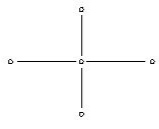
\includegraphics{img/1.jpg}

Разностный уравнения для внутренних узлов сетки:

$${U_m^{p+1}-2U_m^p+U_m^{p-1} \over \tau^2} - {a^2(U_{m+1}^p-2U_m^p+U_{m-1}^p) \over h^2} = f_m^p$$

Где:
\begin{itemize}
    \item $p=1,2,...;$
    \item $m=1,2,...,M-1$
\end{itemize}

Аппроксимация краевых условий:

$$ U_0^p = \Psi_1(t_p), \qquad U_M^p=\Psi_2(t_p)$$

Где:
\begin{itemize}
    \item $p=1,2,...$
\end{itemize}

Аппроксимация начальных условий:

$$U_m^0=\Phi_1(x_m), \qquad {U_m^1-U_m^0 \over \tau} = \Phi_2(x_m)$$

Где:
\begin{itemize}
    \item $m=1,2,...,M$
\end{itemize} 
\textbf{3. Неявная схема (1) (шаблон)}

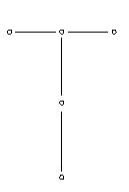
\includegraphics{img/2.jpg}

Разностные уравнения для внутренних узлов сетки:

$${U_m^{p+1}-2U_m^p+U_m^{p-1} \over \tau^2} - {a^2(U_{m+1}^{p+1}-2U_m^{p+1}+U_{m-1}^{p+1}) \over h^2} = f_m^{p+1}$$

Где:
\begin{itemize}
    \item $p=1,2,...; $
    \item $ m=1,2,...,M-1 $
\end{itemize}

Аппроксимация краевых условий:

$$ U_0^p = \Psi_1(t_p), \qquad U_M^p=\Psi_2(t_p)$$

Где:
\begin{itemize}
    \item $p=1,2,...$
\end{itemize}

Аппроксимация начальных условий:

$$U_m^0=\Phi_1(x_m), \qquad {U_m^1-U_m^0 \over \tau} = \Phi_2(x_m)$$

Где:
\begin{itemize}
    \item $m=1,2,...,M$
\end{itemize}

Абсолютно устойчива, но практически не используется, т.к. дает слишком грубые результаты.

\newpage

\section{Выбор шагов по $\tau$ и $h$, точность, устойчивость}

\textbf{1. Дифференциальная краевая задача}

$$U_{tt}-c^2U_{xx}=f(t,x)$$

$$U(t,0)=\psi_1(t)$$

$$U(t,l)=\psi_2(t)$$

$$U(0,x)=\psi_1(x)$$

$$U'(0,x)=\psi_2(x)$$
\textbf{2. Сеточная область}

$$W^h=[(t_p,x_m)], \qquad p=0,1,...,P \qquad m=0,1,...,M$$

$$u^h=[u_m^p], \qquad p=0,1,...,P \qquad m=0,1,...,M$$

где $u_m^p$ - компонента сеточной функции, относящаяся к узлу $(t_p,x_m)$, $t_p=p\tau$, где $\tau$ - шаг по времени, $P\tau=T$, $x_m=mh$, $h$ - шаг по координате, $Mh=1$ \\
\textbf{3. "Крест"} \\
\textbf{3.1 Невязка}

Выберем в качестве опорной точку $(t_p,x_m)$, для разностной схемы "Крест" представим значения $[u(t,x)]$, входящие в выражение для $\partial{f_m^p}$ в виде разложения в ряд Тейлора относительно этой точки.

$$u_m^{p+1}=u_m^p + {\partial{u_m^p \over \partial{t}}\tau} + {1 \over 2!}{\partial^2{u_m^p \over \partial{t^2}}\tau^2} + {1 \over 3!}{\partial^3{u_m^p \over \partial{t^3}}\tau^3} + O(\tau^4) $$

$$u_m^{p-1}=u_m^p - {\partial{u_m^p \over \partial{t}}\tau} + {1 \over 2!}{\partial^2{u_m^p \over \partial{t^2}}\tau^2} - {1 \over 3!}{\partial^3{u_m^p \over \partial{t^3}}\tau^3} + O(\tau^4) $$

$$u_{m+1}^p=u_m^p + {\partial{u_m^p \over \partial{x}}h} + {1 \over 2!}{\partial^2{u_m^p \over \partial{x^2}}h^2} + {1 \over 3!}{\partial^3{u_m^p \over \partial{x^3}}h^3} + O(h^4) $$

$$u_{m-1}^p=u_m^p - {\partial{u_m^p \over \partial{x}}h} + {1 \over 2!}{\partial^2{u_m^p \over \partial{x^2}}h^2} - {1 \over 3!}{\partial^3{u_m^p \over \partial{x^3}}h^3} + O(h^4) $$

$$\partial{f_m^p}={U_m^{p+1}-2U_m^p+U_m^{p-1} \over \tau^2} - c^2{U_{m+1}^p-2U_m^p+U_{m-1}^p \over h^2} - f_m^p $$

$${U_m^{p+1}-2U_m^p+U_m^{p-1} \over \tau^2} = {{1 \over 2!}{\partial^2 {u_m^p} \over \partial{x^2}}h^2 + O(h^4) + {1 \over 2!}{\partial^2 {u_m^p} \over \partial{x^2}} h^2 + O(h^4) \over h^2 } = {{\partial^2 {u_m^p} \over \partial{x^2}} h^2 + O(h^4) \over h^2} = {\partial^2 {u_m^p} \over \partial{x^2}}  + O(h^2) $$

$$\partial{f_m^p}= ({{\partial^2 {u_m^p} \over \partial{t^2}} - c^2 {\partial^2 {u_m^p} \over \partial{x^2}} - f_m^p }) + O(\tau^2+h^2)$$

Таким образом, порядок аппроксимации $||\partial{f_m^p}||=O(\tau^2+h^2)$. Однако в данном варианте схемы второе начальное условие аппроксимируется простейшим образом - с первым порядком точности (по $t$). Поэтому в целом это схема первого порядка. Порядок аппроксимации $||\partial{f_m^p}||=O(\tau+h^2)$.

Соответственно точность решения задачи будет зависеть от величины $\tau+h^2$. Т.е. чтобы получить решение с точностью порядка $\epsilon$, нужно выбрать такие $\tau$, $h$, что $\tau+h^2 \leq A\epsilon$, $A$ - скорость сходимости решения, линейная по времени и квадратичная по координате. \\
\textbf{3.2 Спектральный признак устойчиости}

Спектральный признак состоит в следующем:
Заменем праую часть разностного уравнения нулем, краевую зачау - задачей Коши, функцию $\varphi_m$ заменяем гармоникой $e^{im\omega}$, и ищем решение  в виде $u_m^p=\lambda^pe^{im\omega}$, где $\omega$ произвольное целое число, $0<\omega<2\pi$, Для устойчивости разностной схемы необходимо, чтобы $|\lambda| \leq 1$.

Итак, $u_m^p=\lambda^pe^{im\omega}$ поставим в разностное уравнени, получим

$$ { \lambda-2+{1\over\lambda} \over \tau^2} - c^2 { e^{-i\omega}-2+e^{i\omega} \over h^2} = 0$$

или

$$\lambda^2-2(1-{2\tau^2c^2 \over h^2}{\omega \over 2})\lambda+1=0$$

Произведение корней этого уравнения равно единице. Если дискриминант $D(\omega)={4\tau^2c^2 \over h^2}{\omega \over 2}$ квадратного уравнения  отрицателен, то корни $\lambda_1(\omega)$, $\lambda_2(\omega)$ комплексно-сопряженные и равны единице по модулю.

Разностная схема устойчива, если выполнено неравентсво $|\lambda|\leq 1$,т.е. когда $ \{\ t,h \}\ $ выраны так, что ${\tau^2c^2 \over h^2} \leq 1$. \\
\textbf{4. Неявная схема (1) сшаблоном} \\
\textbf{4.1. Неввязка}

Выберем в качестве опорной точку $(t_p,x_m)$, для разностной схемы "Неявна схема (1) с шаблоном" и представим значения $[u(t,x)]$, входящие в выражение для $\partial{f_m^p}$ в виде разложения в ряд Тейлора относительно точки.

$$u_m^{p+1}=u_m^p + {\partial{u_m^p} \over \partial{t}}\tau + {1 \over 2!}{\partial^2{u_m^p} \over \partial{t^2}}\tau^2 + {1 \over 3!}{\partial^3{u_m^p} \over \partial{t^3}}\tau^3 + O(\tau^4)$$

$$u_m^{p-1}=u_m^p - {\partial{u_m^p} \over \partial{t}}\tau + {1 \over 2!}{\partial^2{u_m^p} \over \partial{t^2}}\tau^2 - {1 \over 3!}{\partial^3{u_m^p} \over \partial{t^3}}\tau^3 + O(\tau^4)$$

$$u_{m-1}^{p+1}=u_m^{p+1} - {\partial{u_m^{p+1}} \over \partial{x}}h + {1 \over 2!}{\partial^2{u_m^{p+1}} \over \partial{x^2}}h^2 - {1 \over 3!}{\partial^3{u_m^{p+1}} \over \partial{x^3}}h^3 + O(h^4)$$

$$u_{m+1}^{p+1}=u_m^{p+1} + {\partial{u_m^{p+1}} \over \partial{x}}h + {1 \over 2!}{\partial^2{u_m^{p+1}} \over \partial{x^2}}h^2 + {1 \over 3!}{\partial^3{u_m^{p+1}} \over \partial{x^3}}h^3 + O(h^4)$$

$$\partial{f_m^p} = {U_m^{p+1}-2U_m^p+U_m^{p-1} \over \tau^2} - c^2{U_{m+1}^{p+1}-2U_m^{p+1}+U_{m-1}^{p+1} \over h^2} - f_m^{p+1}$$

$${U_m^{p+1}-2U_m^p+U_m^{p-1} \over \tau^2} = {{1 \over 2!}{\partial^2{u_m^p} \over \partial{t^2}}\tau^2 + O(\tau^4) + {1 \over 2!}{\partial^2{u_m^p} \over \partial{t^2}}\tau^2 + O(\tau^4) \over \tau^2} = {{\partial^2{u_m^p} \over \partial{t^2}}\tau^2 + O(\tau^4) \over \tau^2} = {\partial^2{u_m^p} \over \partial{t^2}} + O(\tau) $$

$${U_{m+1}^{p+1}-2U_m^{p+1}+U_{m-1}^{p+1} \over h^2} = {{1 \over 2!}{\partial^2{u_m^{p+1}} \over \partial{x^2}}h^2 + O(h^4) + {1 \over 2!}{\partial^2{u_m^{p+1}} \over \partial{x^2}}h^2 + O(h^4) \over \tau^2} = {{\partial^2{u_m^{p+1}} \over \partial{x^2}}h^2 + O(h^4) \over h^2} = {\partial^2{u_m^{p+1}} \over \partial{x^2}} + O(h^2)$$

$$\partial{f_m^p} = ({\partial^2{u_m^p}\over \partial{t^2}} - c^2{\partial^2{u_m^{p+1}} \over \partial{x^2}} - f_m^{p+1}) + O(\tau + h^2)$$

Таким образом, порядок аппроксимации $||\partial{f_m^p}||=O(\tau+h^2)$. \\
\textbf{4.2. Спектральный признак устойчивости}

$u_m^p=\lambda^pe^{im\omega}$ подставим в разностное уравнение, получим

$${\lambda^{p+1}e^{im\omega}-2\lambda^pe^{im\omega}+\lambda^{p-1}e^{im\omega} \over \tau^2} - c^2{\lambda^{p+1}e^{i(m+1)\omega}-2\lambda^{p+1}e^{im\omega}+\lambda^{p+1}e^{i(m-1)\omega} \over h^2} = 0$$

$${\lambda-2+{1\over\lambda} \over \tau^2} - c^2\lambda{e^{-i\omega}-2+e^{i\omega} \over h^2} = 0$$

$$(\lambda-2+{1\over\lambda}) - {c^2\tau^2\lambda \over h^2}(\cos{\cos{\omega}}-2) = 0 $$

$$(\lambda^2-2\lambda+1) - {c^2\tau^2\lambda^2 \over h^2}(\cos{\cos{\omega}}-2) = 0 $$

$$\lambda^2(1-{c^2\tau^2 \over h^2}(\cos{\cos{\omega}}-2)) - 2\lambda + 1 = 0$$

$$a = (1-{c^2\tau^2 \over h^2}(\cos{\cos{\omega}}-2)) \geq 1$$

$D=4-4a>0$, если $a<1$, что невозможно. При $D=0$

$$a = (1-{c^2\tau^2 \over h^2}(\cos{\cos{\omega}}-2)) = 1$$

$${c^2\tau^2 \over h^2} = 0$$

Тогда

$$\lambda^2 - 2\lambda + 1 = 0$$

$$\lambda_1(\omega) = \lambda_2(\omega) = 1$$

Если $D<0$ $\lambda_1(\omega)$, $\lambda_2(\omega)$ комплексно-сопряженные и меньше единицы по модулю.

Значит схема устойчива при любых ${c^2\tau^2 \over h^2}$.

\newpage

\section{Решение в MATLAB}

Струна конечной длины. Оба конца струны закреплены. Струна находится в поле распределенной переменной силы, меняющейся по закону: $F(t, x) = ae^{-\frac{(x-x_0)^2}{\gamma^2}}$. \\
Параметры: плотность струны $\rho$, натяжение струны $T$, длина струны $l$, амплитуда $a$, точка приложения силы $x_0$ (внутри стрнуы) и характерная ширина ее распределния $\gamma$.

Возьмем следующие параметры:
\begin{itemize}
    \item Точка приложения силы: $ x_0 = 0.5 $ (м)
    \item Линейная плотность: $ \rho_l = 0.05 $ (кг/м)
    \item Характерная ширина распределения: $ \gamma = 2.5 $ (м)
    \item Амплитуда: $ a = 0.5 $
\end{itemize}

Тогда  наша функция $ f(t,x) $ будет иметь вид:

$$
    f(t,x) = 0.5 e^{-\frac{(x - 0.5)^2}{2.5^2}}
$$

Граничные условия:

\begin{itemize}
    \item $ U(t, 0) = 0 $
    \item $ U(t, l) = 0 $
\end{itemize}

Начальные условия:

\begin{itemize}
    \item $ U(0, x) = \sin{\pi x} $
    \item $ U'_t(0, x) = 0 $
\end{itemize}

\newpage

Используем схему "Крест": \\

\lstinputlisting{code/string.m}

\newpage

Результат:

\begin{figure}[h]
    \begin{center}
    \begin{minipage}[h]{0.4\linewidth}
    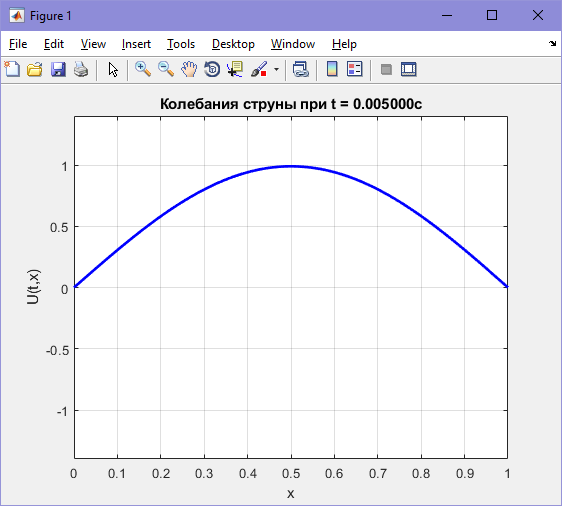
\includegraphics[width=1\linewidth]{img/result_1.png}
    \caption{} %% подпись к рисунку
    \label{ris:experimoriginal}
    \end{minipage}
    \end{center}
\end{figure}

\begin{figure}[h]
    \begin{center}
    \begin{minipage}[h]{0.4\linewidth}
    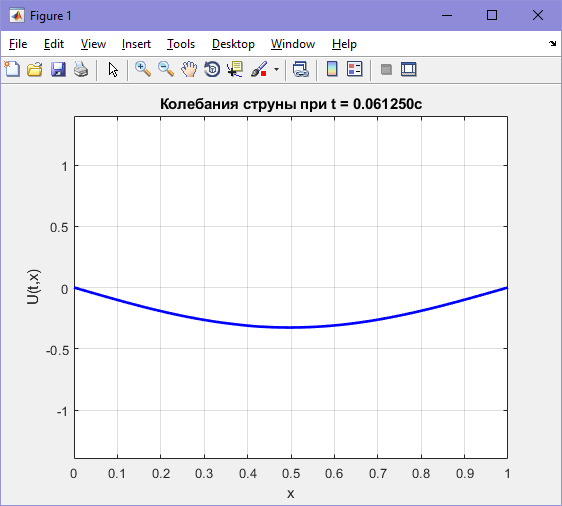
\includegraphics[width=1\linewidth]{img/result_2.png}
    \caption{} %% подпись к рисунку
    \label{ris:experimoriginal}
    \end{minipage}
    \end{center}
\end{figure}

\begin{figure}[]
    \begin{center}
    \begin{minipage}[h]{0.4\linewidth}
    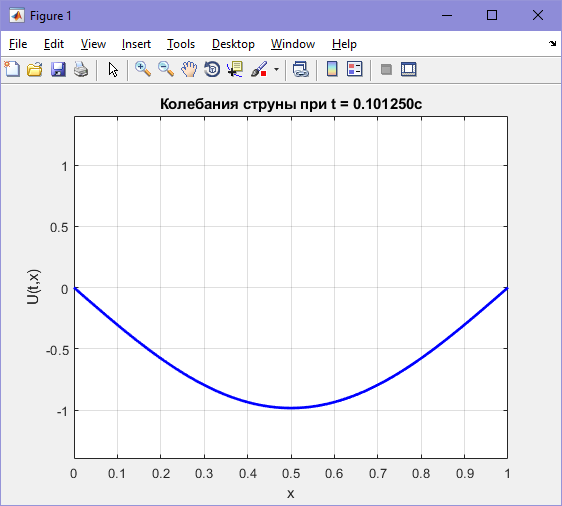
\includegraphics[width=1\linewidth]{img/result_3.png}
    \caption{} %% подпись к рисунку
    \label{ris:experimoriginal}
    \end{minipage}
    \end{center}
\end{figure}

\begin{figure}[]
    \begin{center}
    \begin{minipage}[h]{0.4\linewidth}
    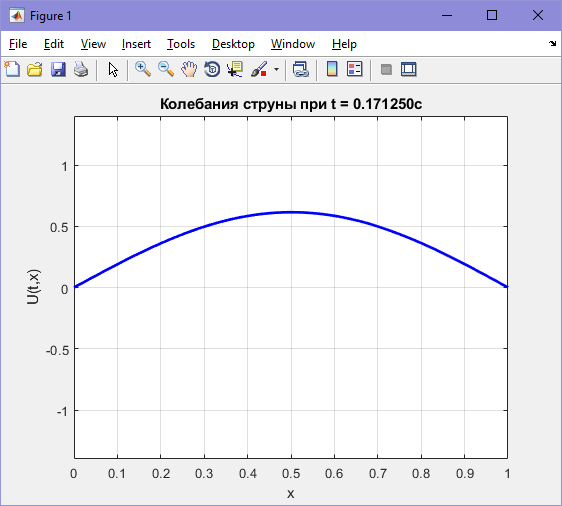
\includegraphics[width=1\linewidth]{img/result_4.png}
    \caption{} %% подпись к рисунку
    \label{ris:experimoriginal}
    \end{minipage}
    \end{center}
\end{figure}

\begin{figure}[]
    \begin{center}
    \begin{minipage}[h]{0.4\linewidth}
    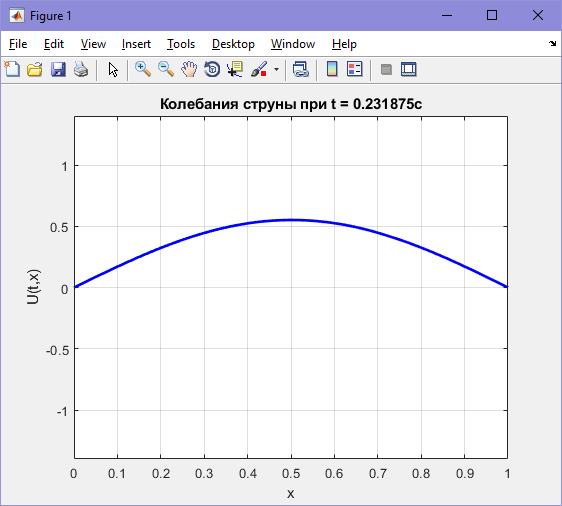
\includegraphics[width=1\linewidth]{img/result_5.png}
    \caption{} %% подпись к рисунку
    \label{ris:experimoriginal}
    \end{minipage}
    \end{center}
\end{figure}





\end{document}
